\begin{figure}[H]
    \centering
    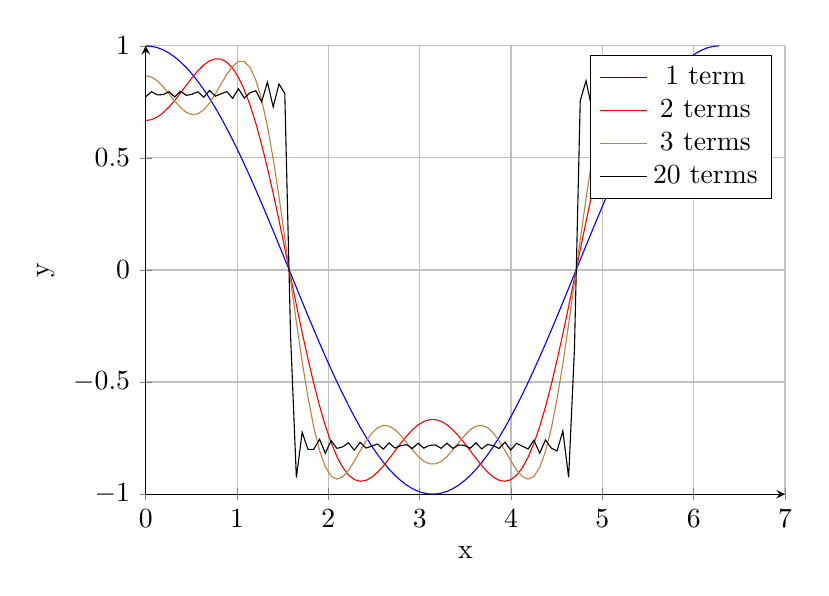
\begin{tikzpicture}
        \begin{axis}[
            width=0.8\textwidth,
            height=0.6\textwidth,
            axis lines = left,
            xlabel = {x},
            ylabel = {y},
            xmajorgrids=true,
            ymajorgrids=true,
            ymin=-1,
            ymax=1,
            xmin=0,
            xmax=7
        ]
            \addplot[
                domain=0:6.28,
                samples=100,
                color=blue
            ] {cos(x*57.2958)};
            \addlegendentry{1 term}

            \addplot[
                domain=0:6.28,
                samples=100,
                color=red
            ] {cos(x*57.2958) - (cos(3*x*57.2958)/3)};
            \addlegendentry{2 terms}

            \addplot[
                domain=0:6.28,
                samples=100,
                color=brown
            ] {cos(x*57.2958) - (cos(3*x*57.2958)/3) + (cos(5*x*57.2958)/5)};
            \addlegendentry{3 terms}

            \addplot[
                domain=0:6.28,
                samples=100,
                color=black
            ] {
                cos(x*57.2958) - 
                (cos(3*x*57.2958)/3) + 
                (cos(5*x*57.2958)/5) - 
                (cos(7*x*57.2958)/7) + 
                (cos(9*x*57.2958)/9) - 
                (cos(11*x*57.2958)/11) + 
                (cos(13*x*57.2958)/13) - 
                (cos(15*x*57.2958)/15) + 
                (cos(17*x*57.2958)/17) - 
                (cos(19*x*57.2958)/19) + 
                (cos(21*x*57.2958)/21) - 
                (cos(23*x*57.2958)/23) + 
                (cos(25*x*57.2958)/25) - 
                (cos(27*x*57.2958)/27) + 
                (cos(29*x*57.2958)/29) - 
                (cos(31*x*57.2958)/31) + 
                (cos(33*x*57.2958)/33) - 
                (cos(35*x*57.2958)/35) + 
                (cos(37*x*57.2958)/37) - 
                (cos(39*x*57.2958)/39)};
            \addlegendentry{20 terms}
        \end{axis}
    \end{tikzpicture}
    \caption{Fourier series approximation of a square wave with varying number of cosine terms. Plotted with pgfplots from functions}
    \label{fig:fourier_series_square_wave_calculated}
\end{figure}